\chapter{Results}\label{ch:results}
\section{Stationarity, height, and sampling}\label{sec:baseline}
\subsection{Approach to the measured regime}\label{sec:stationarity}
The pilot resolves initial mass accumulation and later fluctuations (Figure~\ref{fig:pilot}). Empty starts give a lower mean in the first $10L^2$-grain window. The longest estimated height or frequency correlation time was about 1,195 grains, making the chosen block about seven times longer. These diagnostics guided burn-in and blocking for the measured observables. Each starting state had one independent pilot chain.

\begin{figure}[!htbp]
\centering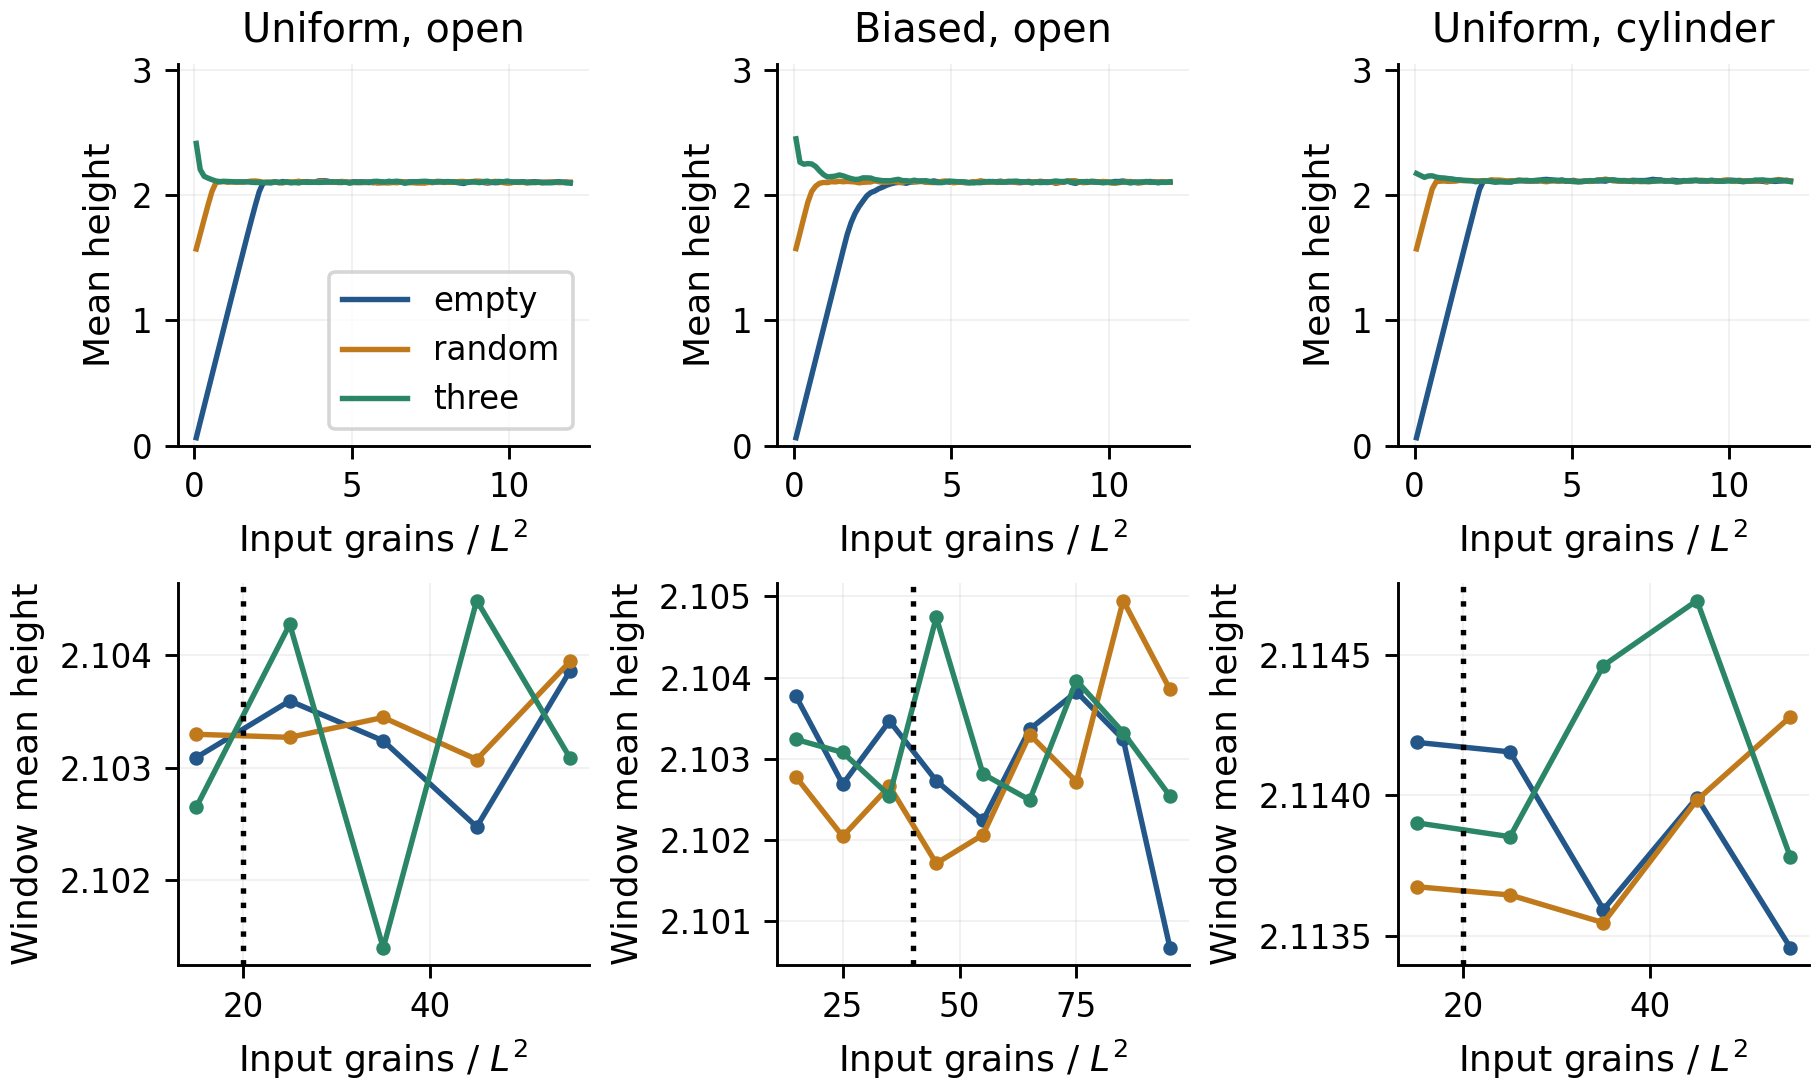
\includegraphics[width=\linewidth]{generated/pilot.png}
\caption{Different initial configurations approach similar late-stage height levels within each model, supporting the selected burn-in for the measured observables. Independent $L=64$ pilots start empty, random stable and all-three. Top: 512-grain mean heights over the first $12L^2$ grains. Bottom: connected $10L^2$-window means after the first window; vertical lines mark selected burn-in. Uniform/cylinder pilots last $60L^2$ grains; biased pilots last $100L^2$. The main runs use independent seeds. These checks do not establish complete mixing.}
\label{fig:pilot}
\end{figure}

Across four consecutive measurement windows, height, all four height frequencies, mean topplings, loss and dissipation probability fluctuate without a common continuing drift. The small height difference under bias prompted a separate investigation (Section~\ref{sec:bias}). Every main run passed the exact mass and potential-balance checks in Eq.~\eqref{eq:potentialbalance}, and every sparse benchmark residual was below $10^{-10}$.

\subsection{Height, finite size, and flux}\label{sec:height}
The equal-height-frequency prediction of $3/2$ is inconsistent with the measured baseline (Table~\ref{tab:baseline}, Figure~\ref{fig:baseline}). Mean height rises from \R{base8height} at $L=8$ to \R{base64height} at $L=64$, approaching the infinite-volume value $17/8$. Height-three sites are much more frequent than height-zero sites.

\begin{table}[!htbp]
\centering\small\setlength{\tabcolsep}{4pt}
\begin{tabular}{@{}rrrrrrr@{}}
\toprule
$L$ & Mean height & Pred. $S$ & Measured $S$ & $P(S=0)$ & $P(D=0\mid S>0)$ & $P(D>0)$ \\
\midrule
8 & $1.98211 \pm 0.00114$ & 3.462 & $3.463 \pm 0.003$ & 0.6194 & 0.2331 & 0.2919 \\
16 & $2.04645 \pm 0.00024$ & 11.338 & $11.333 \pm 0.018$ & 0.5910 & 0.3883 & 0.2502 \\
32 & $2.08355 \pm 0.00044$ & 40.580 & $40.611 \pm 0.066$ & 0.5743 & 0.5245 & 0.2024 \\
64 & $2.10361 \pm 0.00025$ & 153.043 & $153.033 \pm 0.426$ & 0.5649 & 0.6373 & 0.1578 \\
\bottomrule
\end{tabular}

\caption{Baseline simulations with five seeds and one million grains per size. Heights and topplings are means $\pm$ 95\% seed-level interval half-widths, averaging over all input events. Predictions come from the sparse systems. The last columns give zero-avalanche probability, zero-loss probability among avalanches, and loss probability per input.}
\label{tab:baseline}
\end{table}

\begin{figure}[!htbp]
\centering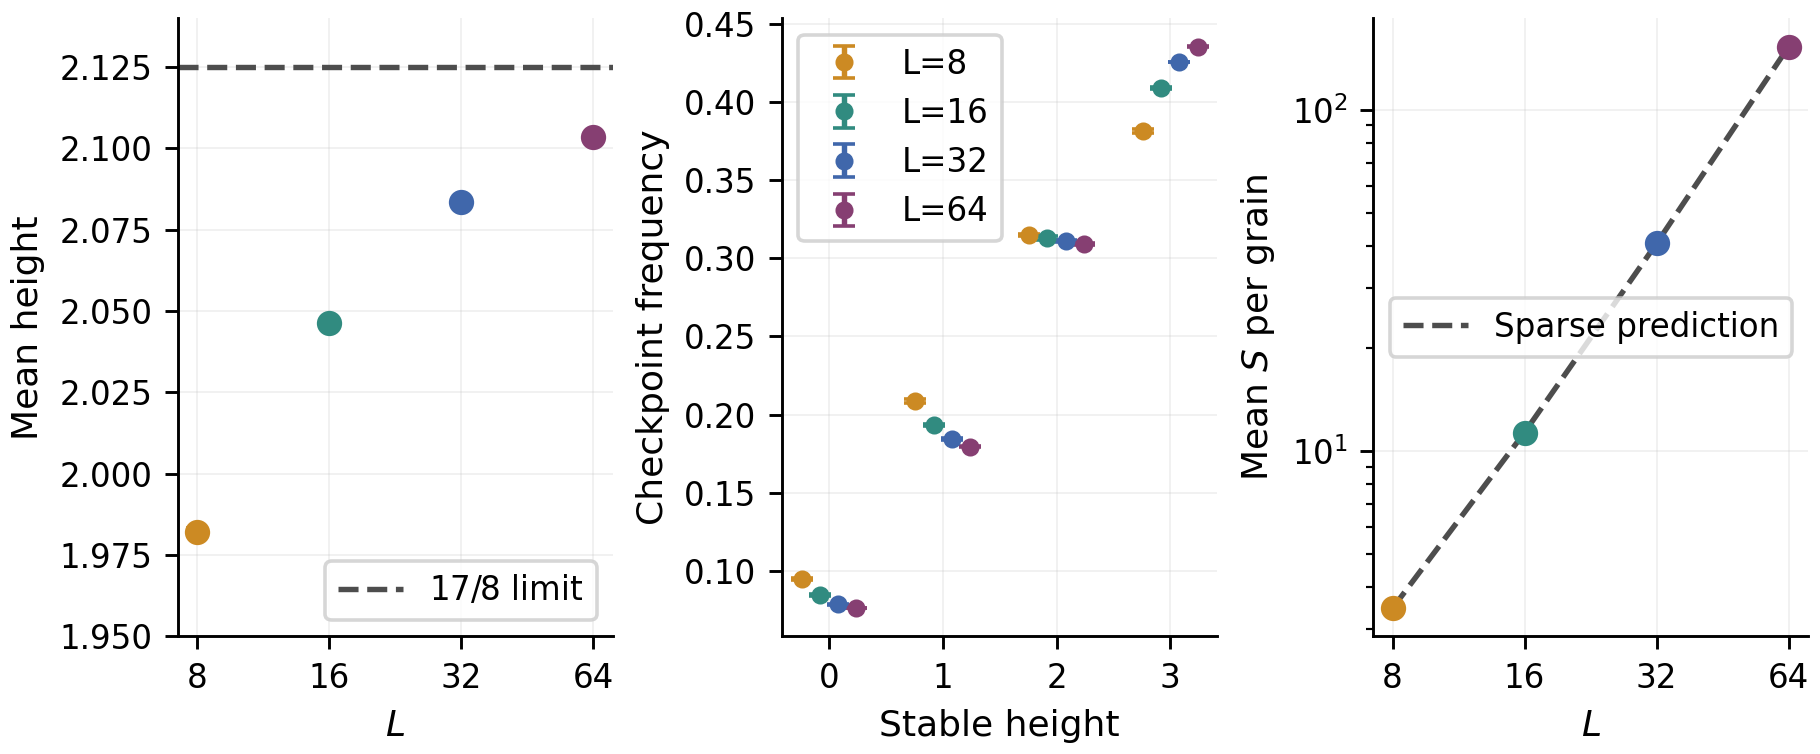
\includegraphics[width=\linewidth]{generated/baseline.png}
\caption{Stable heights have unequal frequencies, mean height increases with $L$, and measured mean topplings agree with finite-grid predictions. Each size uses one million measured inputs across five seeds. Left: mean height and the $17/8$ infinite-volume reference. Centre: height frequencies after stabilization at regular intervals. Right: all-input mean topplings and independent predictions. Error bars are 95\% seed intervals; some are smaller than the markers.}
\label{fig:baseline}
\end{figure}

At $L=64$, mean topplings are \R{base64S_grain}, with interval $\R{base64S_grainCI}$ containing the prediction \R{base64prediction}. All four baseline sizes agree with their finite-grid benchmarks at the reported precision. Mean loss per grain is \R{base64D_grain}, with interval $\R{base64D_grainCI}$; the endpoint mass accounts exactly for its small departure from one. As $L$ increases, loss occurs less often but dissipative events lose more grains: $\E[D\mid D>0]$ rises from \R{base8D_positive} to \R{base64D_positive}. Larger grids carry roughly the same mean flux through rarer, larger loss events.

\subsection{Time versus independent ensemble}\label{sec:sampling}
For $L=32$, one long trajectory gives time-sampled mean height \R{timeheight}, interval $\R{timeheightCI}$, and height-three fraction \R{timep3}, interval $\R{timep3CI}$. Sampling 100 independent chains after $20L^2$ inputs gives \R{ensembleheight}, interval $\R{ensembleheightCI}$, and \R{ensemblep3}, interval $\R{ensemblep3CI}$, respectively. The intervals overlap. At the earlier ages of $L^2$ and $2L^2$ inputs, the ensemble summaries still show the effect of starting empty.

\begin{figure}[!htbp]
\centering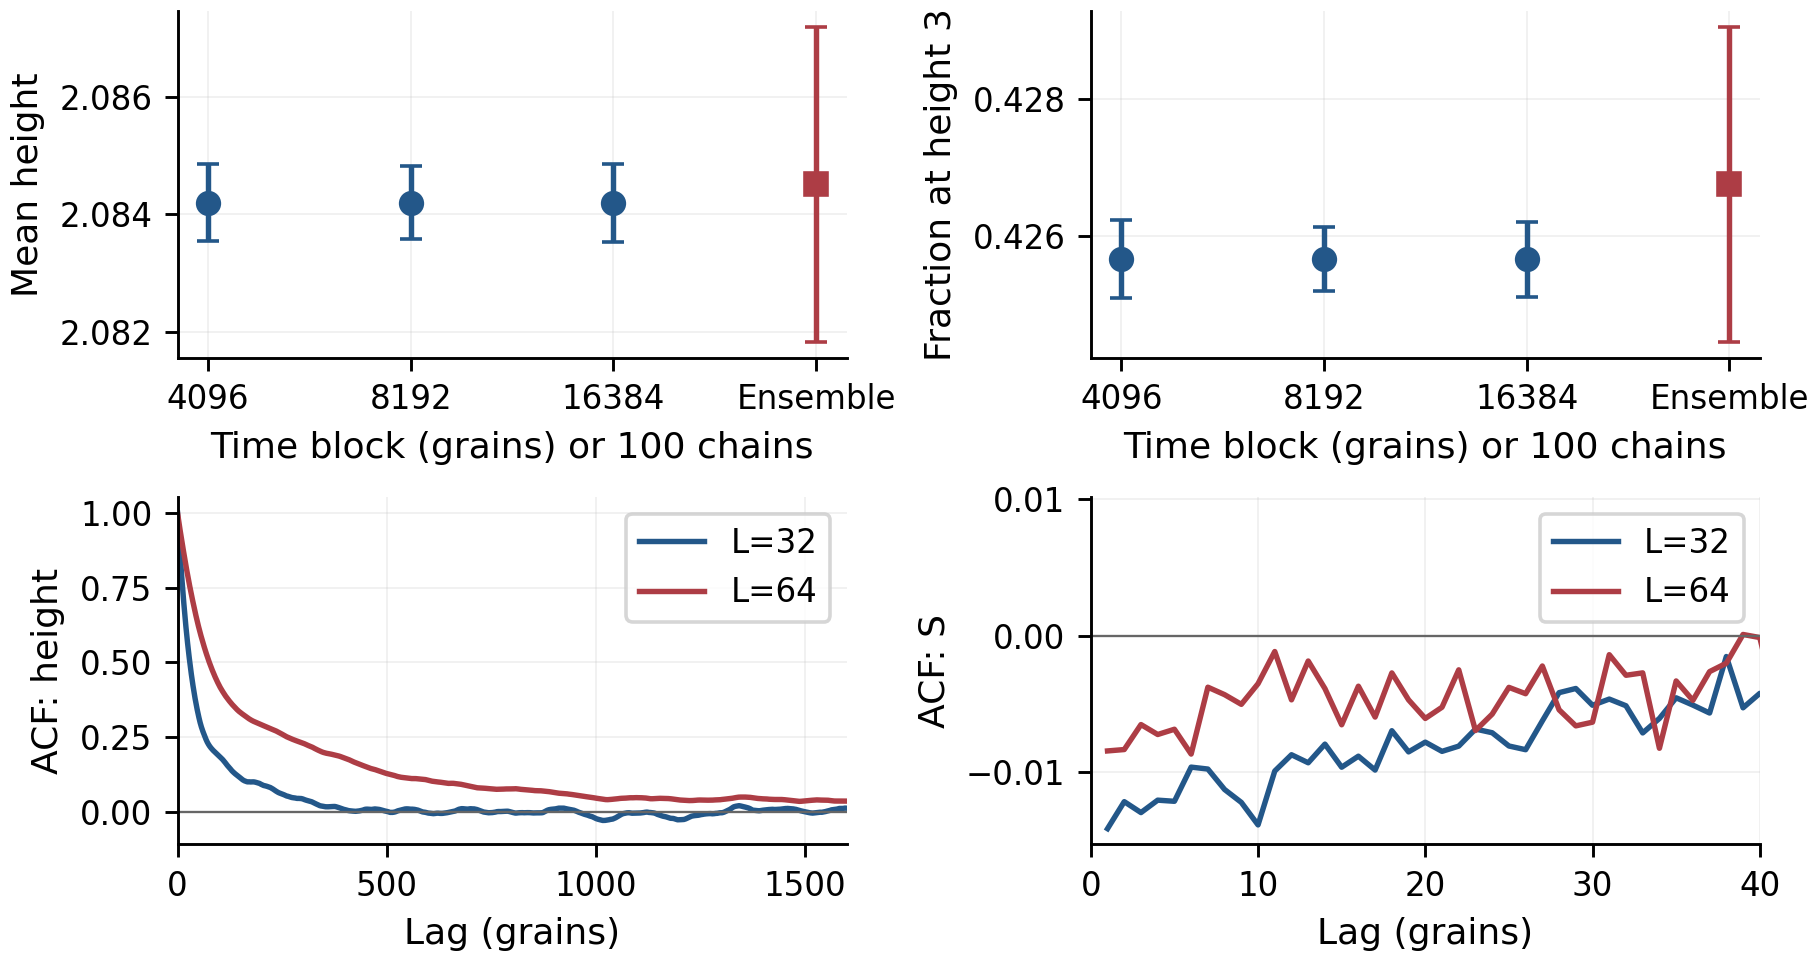
\includegraphics[width=\linewidth]{generated/sampling.png}
\caption{Time and ensemble sampling. Top: estimates and 95\% intervals from one $L=32$ trajectory at three block lengths, compared with 100 independent chains at age $20L^2$. Time estimates cover 196,608 grains, with height-three frequency sampled every 128 grains. Bottom: height and toppling ACFs for the first run at $L=32,64$. The different dependence patterns motivate separate diagnostics for each observable. The ensemble unit is an independent chain.}
\label{fig:sampling}
\end{figure}

The time and ensemble estimates remain consistent when the block length changes. Height has persistent positive dependence, whereas topplings show short-lag anticorrelation. These different patterns support using separate dependence diagnostics for each observable.

\section{Avalanche distributions and finite-range fits}\label{sec:distributions}
At $L=64$, the largest observed toppling count is \R{fitSpowermax}, above the fitting cap $L^2=4096$. These larger events remain in the means and empirical distributions (Figure~\ref{fig:distributions}). The bounds $L^2$ for area and $2L-1$ for single-source open reach reflect the finite grid directly. Loss measures transport to the boundary and differs in distribution from topples or area.

\begin{figure}[!htbp]
\centering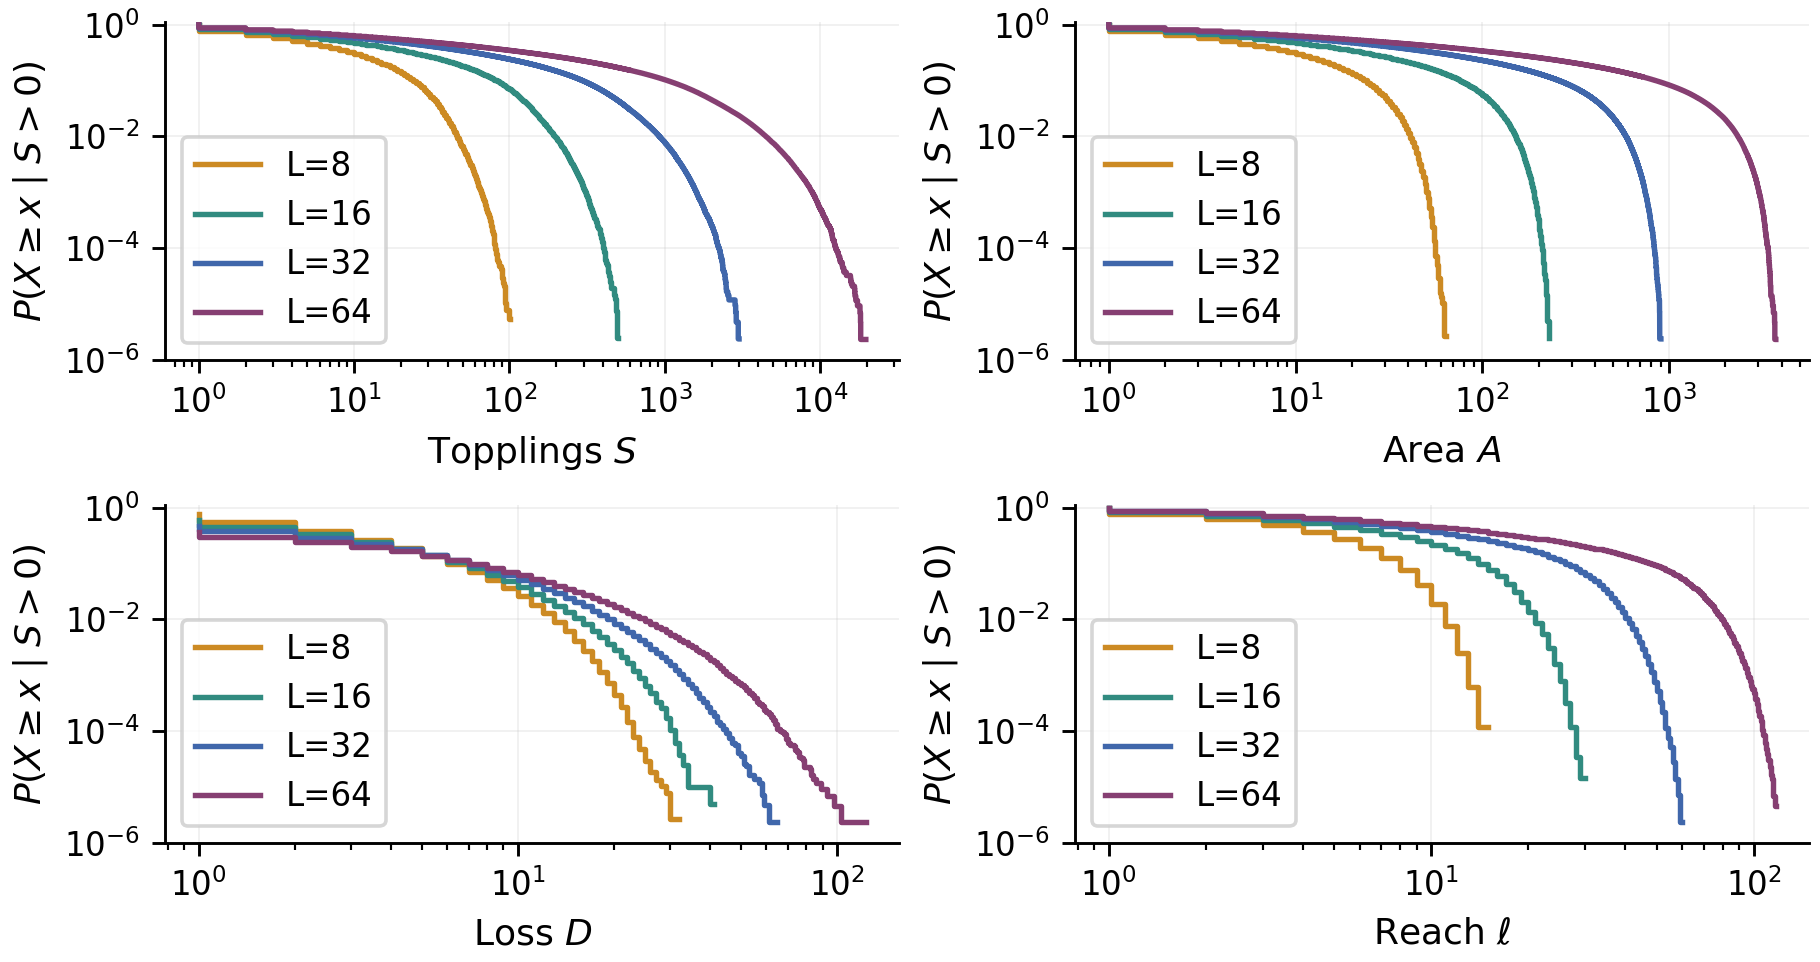
\includegraphics[width=\linewidth]{generated/distributions.png}
\caption{Avalanches extend to larger sizes as $L$ grows, with different shapes for topplings, area, loss and reach. Baseline CCDFs use $L=8,16,32,64$, five seeds and one million inputs per size, conditional on $S>0$. Left-continuous steps show inclusive $P(X\geq x)$. Zero loss remains in the normalization but is absent on log axes; Table~\ref{tab:baseline} gives its mass. Broad ranges alone do not establish universal power laws.}
\label{fig:distributions}
\end{figure}

Zero events make a substantial part of the sample. At $L=64$, $P(S=0)=\R{base64p_zero}$, and $P(D=0\mid S>0)=\R{base64p_zero_loss_given_avalanche}$. A positive-loss tail describes only the dissipative subset of avalanches.

\begin{samepage}
The mean $\E[S]$ in Eq.~\eqref{eq:benchmark} averages over every input, including those that cause no toppling.\par
\end{samepage}

\begin{table}[!htbp]
\centering\small\setlength{\tabcolsep}{4pt}
\begin{tabular}{@{}llrrrr@{}}
\toprule
Quantity: support & Model & Retained $n$ & $\alpha$ & $\lambda$ & KS \\
\midrule
$S$: [16,4096] & Power & 245,477 & $1.1426 \pm 0.0024$ & -- & 0.0310 \\
 & Cutoff & 245,477 & $1.0090 \pm 0.0082$ & $0.000312 \pm 0.000016$ & 0.0074 \\
 & Exp. & 245,477 & -- & $0.002109 \pm 0.000011$ & 0.2468 \\
$A$: [8,4096] & Power & 291,321 & $1.1354 \pm 0.0017$ & -- & 0.0461 \\
 & Cutoff & 291,321 & $0.9591 \pm 0.0023$ & $0.000537 \pm 0.000007$ & 0.0185 \\
 & Exp. & 291,321 & -- & $0.002783 \pm 0.000018$ & 0.2717 \\
$D$: [1,12289] & Power & 157,789 & $1.5098 \pm 0.0031$ & -- & 0.2242 \\
 & Cutoff & 157,789 & $0.2627 \pm 0.0312$ & $0.1365 \pm 0.0037$ & 0.0247 \\
 & Exp. & 157,789 & -- & $0.1718 \pm 0.0009$ & 0.0468 \\
$\ell$: [3,127] & Power & 345,680 & $1.2171 \pm 0.0039$ & -- & 0.0713 \\
 & Cutoff & 345,680 & $0.5817 \pm 0.0040$ & $0.0293 \pm 0.0002$ & 0.0260 \\
 & Exp. & 345,680 & -- & $0.0529 \pm 0.0003$ & 0.0895 \\
\bottomrule
\end{tabular}

\caption{Discrete marginal fits at $L=64$, using identical support for the three models within each observable. Parameters are means $\pm$ 95\% half-widths across five independent seed fits; $n$ is the total retained count, and KS is the mean descriptive CDF discrepancy. Power fixes $\lambda=0$ and exponential fixes $\alpha=0$. The $S$ cap selects an intermediate range; other caps are physical bounds. Loss fits condition on $D>0$; the other fits use their displayed positive intervals.}
\label{tab:fits}
\end{table}

On $16\leq S\leq4096$, the pure-power effective exponent is \R{fitSpoweralpha}, with interval $\R{fitSpoweralphaCI}$. Adding an exponential cutoff reduces mean KS from \R{fitSpowerKS} to \R{fitScutoffKS}; an exponential alone gives \R{fitSexponentialKS}. The cutoff model gains \R{fitScutoffscore} nats per retained observation in mean marginal log score over power. Its CDF follows the observed curvature more closely on this range. The comparison is descriptive because the scores use the fitting data and the cutoff model has an extra parameter.

\begin{figure}[!htbp]
\centering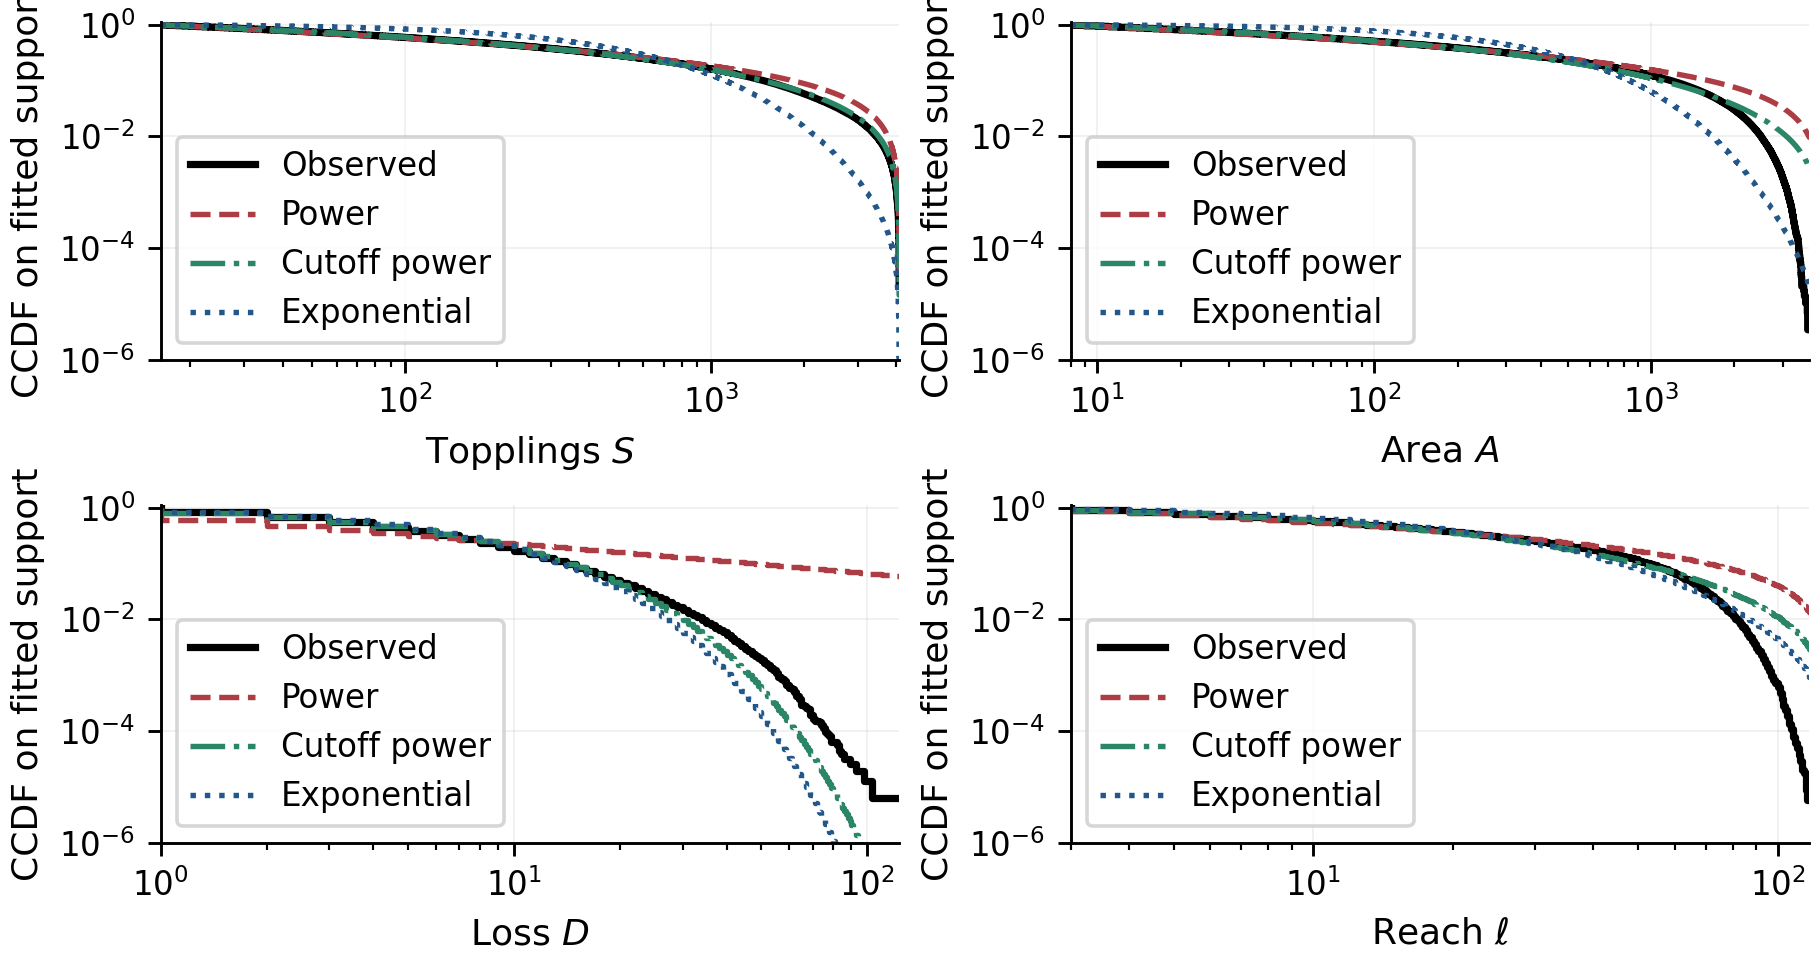
\includegraphics[width=\linewidth]{generated/fits.png}
\caption{Observed and fitted CCDFs at $L=64$, conditional on the intervals in Table~\ref{tab:fits}. Observed curves pool the five equal-length runs. Model curves average the five separately normalized fitted PMFs before cumulation. Normalization uses the full fitting support, even where the display stops near the observed maximum. Cutoff models follow the curves more closely, with some systematic residual shape.}
\label{fig:fits}
\end{figure}

Area also shows curvature: the power and cutoff KS distances are \R{fitApowerKS} and \R{fitAcutoffKS}. For positive loss, a pure power gives KS \R{fitDpowerKS}, compared with \R{fitDexponentialKS} for an exponential and \R{fitDcutoffKS} for cutoff power. Reach has a visibly curved finite-support distribution too. The four observables therefore support finite-range descriptions with different shapes.

The estimated slopes depend on the fitting range. At $L=64$, halving and doubling the chosen lower limits gives pure-power estimates spanning \R{sensitivityS} for $S$, \R{sensitivityA} for area, \R{sensitivityD} for positive loss and \R{sensitivityell} for reach. This variation is separate from the narrower uncertainty intervals conditional on one range. Broad distributions and growing scales match the expected BTW behaviour, but the range dependence limits interpretation of a single fitted exponent. Earlier work also found that simple scaling fails for BTW toppling statistics~\cite{demenech1998}.

An additional upper-limit check uses the same five $L=64$ runs and $x_{\min}=16$, with $x_{\max}=2048,4096,8192$. The retained counts are \R{upperRetained}, respectively. Mean cutoff KS distances are \R{uppercutoffKS}, compared with \R{upperpowerKS} for power, and pure-power exponents span \R{upperPowerAlpha}. Curvature is preferred descriptively at all three caps, while the parameter estimates remain range-dependent.

\section{Correlations and the role of the source position}\label{sec:correlations}
We expected a positive correlation between $S$ and $A$: every site counted in the area must topple at least once, and some sites topple repeatedly. Larger areas should also tend to have greater spatial extent. Loss should depend on these quantities as well as distance from the input site to the boundary. Figure~\ref{fig:correlations} supports these predictions. All six Spearman correlations use $S>0$ and retain zero-loss avalanches.

At $L=64$, $\rho(S,A)=\R{rhoSA}$ with interval $\R{rhoSACI}$, $\rho(S,\ell)=\R{rhoSell}$ with $\R{rhoSellCI}$, and $\rho(A,\ell)=\R{rhoAell}$ with $\R{rhoAellCI}$. Repeated topplings and differences in cluster shape allow these observables to differ even when their ranks agree closely. Loss is less strongly correlated: $\rho(S,D)=\R{rhoSD}$ with $\R{rhoSDCI}$, $\rho(A,D)=\R{rhoAD}$ with $\R{rhoADCI}$, and $\rho(D,\ell)=\R{rhoDell}$ with $\R{rhoDellCI}$.

\begin{figure}[!htbp]
\centering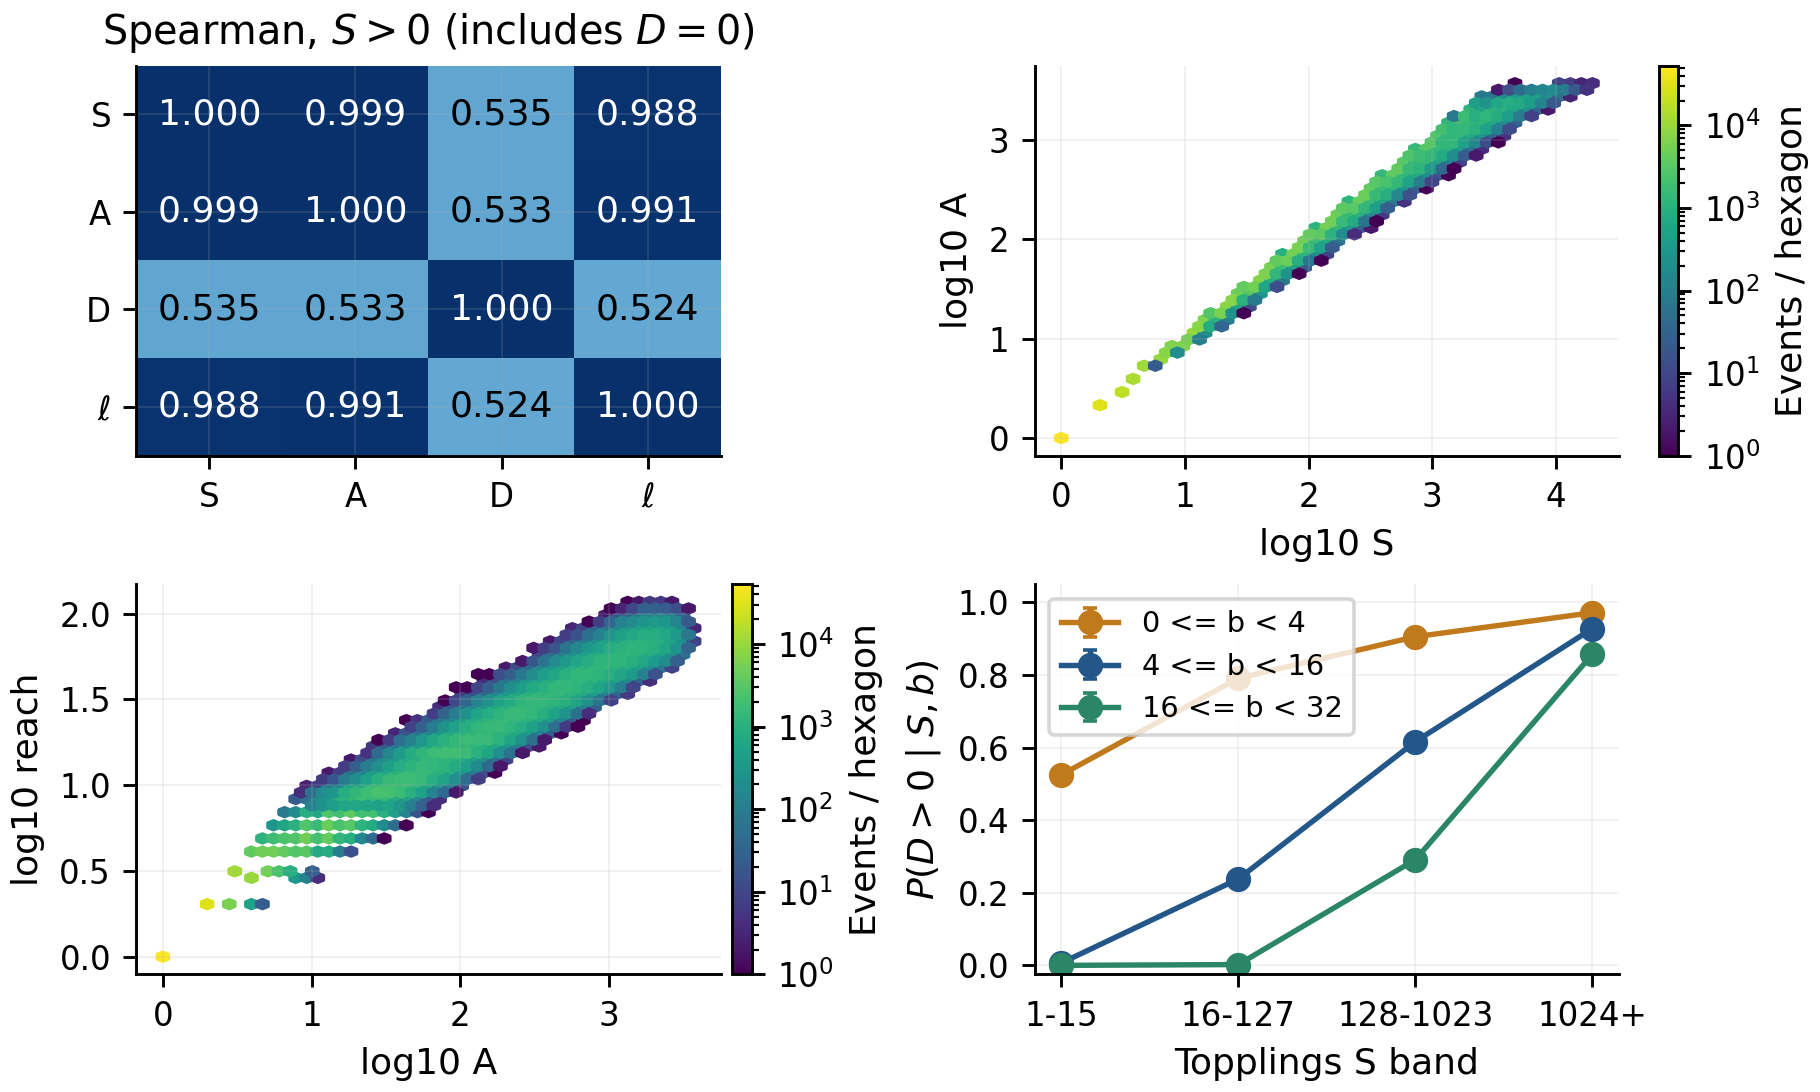
\includegraphics[width=\linewidth]{generated/correlations.png}
\caption{Size, area and reach track one another closely; loss depends more on sink access. Baseline $L=64$ uses \R{base64avalancheN} nonzero avalanches across five seeds, retaining $D=0$. Top left: mean seed Spearman matrix. Top right and bottom left: joint log-coordinate counts for the full nonzero sample; colour gives events per hexagon. Bottom right: loss probability within fixed size bands and source boundary-distance $b$ strata, with 95\% seed intervals.}
\label{fig:correlations}
\end{figure}

The boundary-distance groups show that avalanches of similar size are more likely to dissipate when they start nearer a sink. Activity from a source farther inside the grid must reach a boundary before any grain can leave. This helps explain why loss correlates less strongly with topples than area does. Other avalanche features still vary within each group. Each grid size is analysed separately.

\section{Controlled changes to drive, boundaries and grouping}\label{sec:extensions}
Table~\ref{tab:extensions} compares each extension with its control at the same size. Open and cylindrical runs receive the same grain budget. Batch runs receive the same total grains in a quarter as many events. In each model, conservation gives stationary mean loss one per grain, while the measurements show how that loss is distributed across events.

\begin{table}[!htbp]
\centering\small\setlength{\tabcolsep}{3.6pt}
\begin{tabular}{@{}rlrrrrr@{}}
\toprule
$L$ & Condition & Mean height & $S$/grain & $P(S>0)$ & $P(D>0)$ & $E[D\mid D>0]$ \\
\midrule
32 & Open/uniform & $2.08355 \pm 0.00044$ & $40.61 \pm 0.07$ & 0.4257 & 0.2024 & 4.941 \\
32 & Open/biased & $2.08297 \pm 0.00050$ & $69.02 \pm 0.06$ & 0.4409 & 0.1396 & 7.166 \\
32 & Cylinder & $2.10369 \pm 0.00059$ & $93.55 \pm 0.12$ & 0.4351 & 0.1687 & 5.927 \\
32 & Batch, $m=4$ & $2.08355 \pm 0.00044$ & $40.61 \pm 0.07$ & 0.8917 & 0.5983 & 6.686 \\
64 & Open/uniform & $2.10361 \pm 0.00025$ & $153.03 \pm 0.43$ & 0.4351 & 0.1578 & 6.337 \\
64 & Open/biased & $2.10313 \pm 0.00048$ & $266.67 \pm 0.19$ & 0.4442 & 0.1035 & 9.662 \\
64 & Cylinder & $2.11401 \pm 0.00053$ & $357.51 \pm 0.09$ & 0.4406 & 0.1271 & 7.869 \\
64 & Batch, $m=4$ & $2.10361 \pm 0.00025$ & $153.03 \pm 0.43$ & 0.8978 & 0.4984 & 8.025 \\
\bottomrule
\end{tabular}

\caption{Comparisons at matched sizes, with five seeds and one million measured grains per row. Mean height and topplings per grain include 95\% seed half-widths. Probabilities and conditional loss use single-grain events for the first three rows at each $L$ and four-grain events for batches. Batch mean loss is near four per event and one per grain. Batch estimates are paired with baseline.}
\label{tab:extensions}
\end{table}

\subsection{Full-support spatial bias}\label{sec:bias}
On the open square, we bias the input towards the centre using
\begin{equation}
 q_\eta(x)=\frac{1-\eta}{L^2}+\eta\,
 \frac{\exp[-\|x-c\|_2^2/(2\sigma^2)]}{\sum_y\exp[-\|y-c\|_2^2/(2\sigma^2)]},
 \quad \eta=0.9,\quad\sigma=L/8,\quad c=((L-1)/2,(L-1)/2).
\end{equation}
Every site has positive input probability, bounded below by $0.1/L^2$. Changing these probabilities on the same graph preserves the recurrent stationary measure and its height statistics. The mean response is $\E[S]=q^\top w$, however, so it weights sites according to their input probabilities. Central sites are farther from sinks and have a larger expected response. Biased input can therefore increase mean topplings while preserving the stationary state measure.

At $L=64$, mean topplings rise from \R{base64S_grain} to \R{bias64S_grain}, close to the actual-$q$ benchmark \R{bias64prediction} (Figure~\ref{fig:driving}). Dissipation probability falls from \R{base64p_loss} to \R{bias64p_loss}, while mean loss conditional on dissipation rises from \R{base64D_positive} to \R{bias64D_positive}. Mean loss per grain is \R{bias64D_grain}. The triggering probability can also change: biased input samples sites with different spatial weights even when the stationary law of the grid stays the same.

\begin{figure}[!htbp]
\centering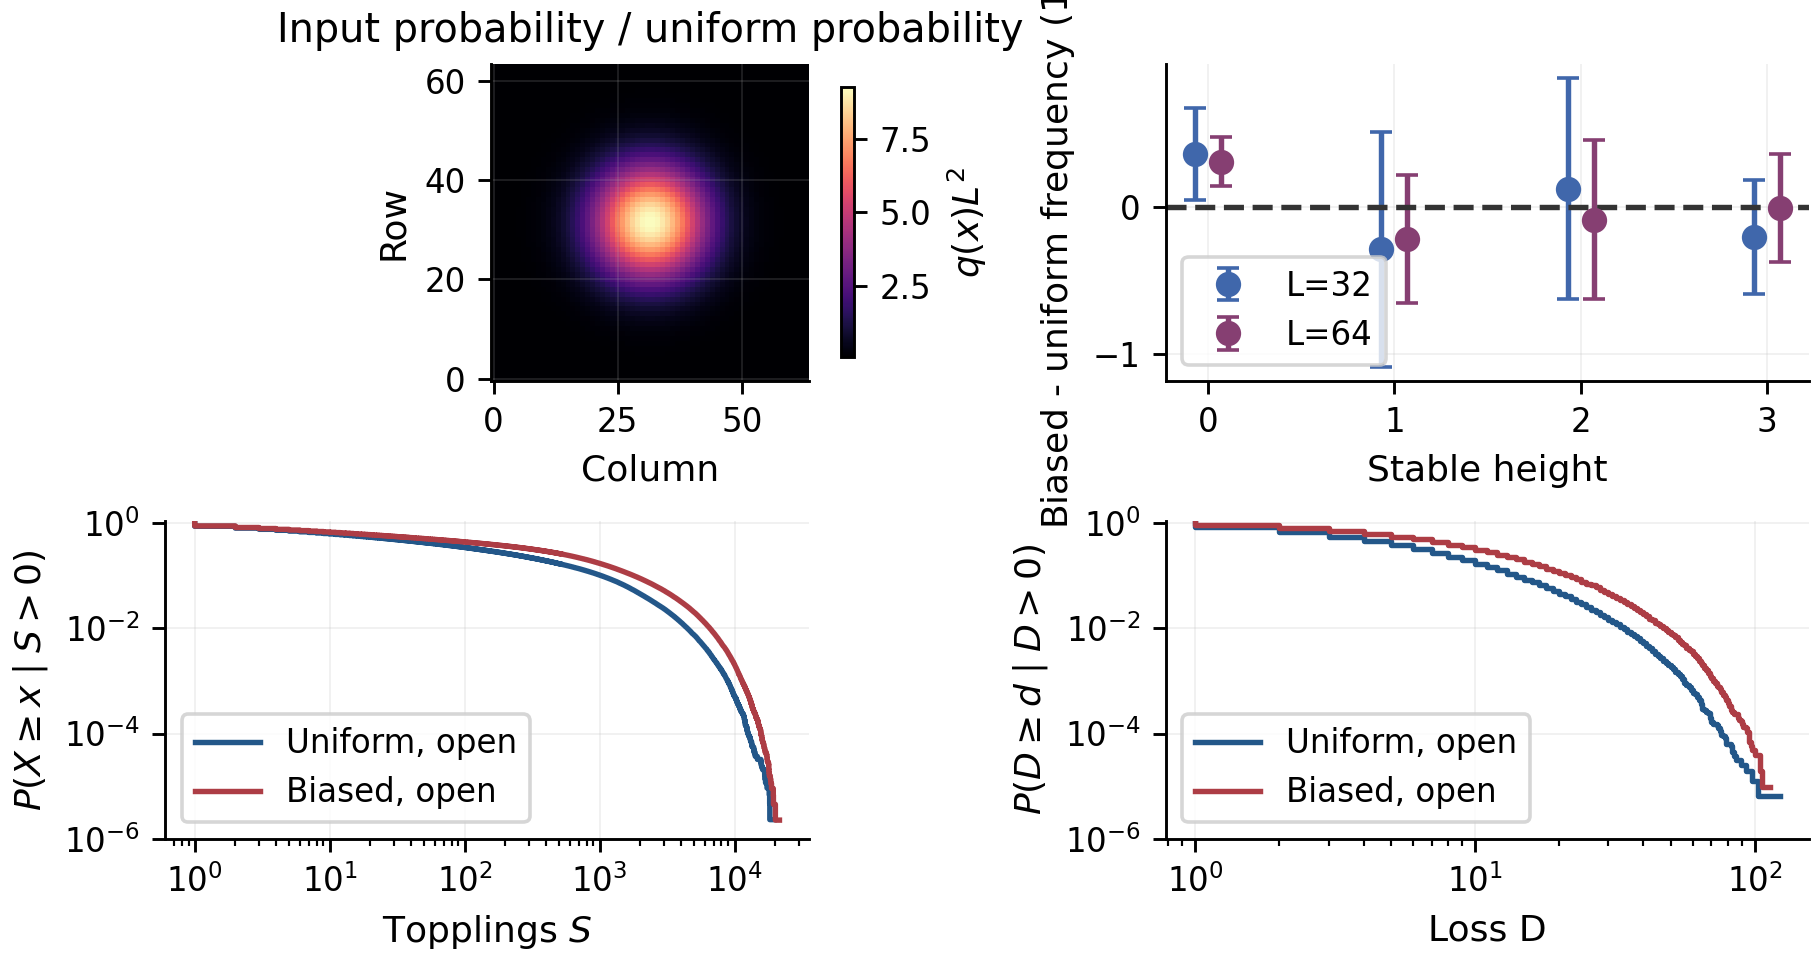
\includegraphics[width=\linewidth]{generated/driving.png}
\caption{Spatial bias changes avalanche responses; the stationary height distribution is theoretically invariant on the same graph under full-support driving. Top left: $L=64$ input probability relative to uniform. Top right: finite-sample biased-minus-uniform height-frequency differences at $L=32,64$, with Welch 95\% independent-seed intervals; the theoretical difference is zero. Bottom: $L=64$ size ($S>0$) and loss ($D>0$) CCDFs, with five seeds per condition.}
\label{fig:driving}
\end{figure}

The initial $L=32$ height difference was \R{bias32heightDifference}, with nominal interval $\R{bias32heightDifferenceCI}$ narrowly excluding zero. At $L=64$ it was \R{bias64heightDifference}, interval $\R{bias64heightDifferenceCI}$. To investigate, we ran a separate confirmation with five new seeds for both models at both sizes, $100L^2$ burn-in and 800,000 measured grains per chain. Each condition received the same larger budget. The differences were \R{confirm32}, interval $\R{confirm32CI}$, and \R{confirm64}, interval $\R{confirm64CI}$, respectively. The longer runs do not reproduce a persistent deficit. With five seeds and several inspected contrasts, the initial nominal interval warrants caution. The confirmation intervals are compatible with zero at the precision of this comparison.

\subsection{Cylindrical boundaries}\label{sec:cylinder}
For the cylinder, columns are periodic and grains leave only above the top row or below the bottom row. At $L\geq3$, a toppling on a dissipative row loses one grain, including at the periodic seam. The simulations use widths of at least three. The graph distance is
\begin{equation}
 d_{\rm cyl}((i,j),(i_0,j_0))=|i-i_0|+\min(|j-j_0|,L-|j-j_0|),
\end{equation}
and the source distance to a dissipative boundary is $\min(i,L-1-i)$. Reach follows this cylindrical distance and is bounded by $L+\lfloor L/2\rfloor$.

A finite-grid benchmark follows by taking $w$ constant along each row. Set $w_{-1}=w_L=0$ and
\begin{equation}
 w(i,j)=\frac{(i+1)(L-i)}{2}.
\end{equation}
The horizontal neighbours cancel two diagonal contributions, giving $(K_{\rm cyl}w)_{i,j}=2w_i-w_{i-1}-w_{i+1}=1$, including on the dissipative rows. Averaging over uniform input yields
\begin{equation}
 \E[S]_{\rm cyl}=\frac1L\sum_{i=0}^{L-1}\frac{(i+1)(L-i)}2
               =\frac{(L+1)(L+2)}{12}.\label{eq:cylinder}
\end{equation}
Substitution into the sparse matrix verifies this analytic result.

\begin{figure}[!htbp]
\centering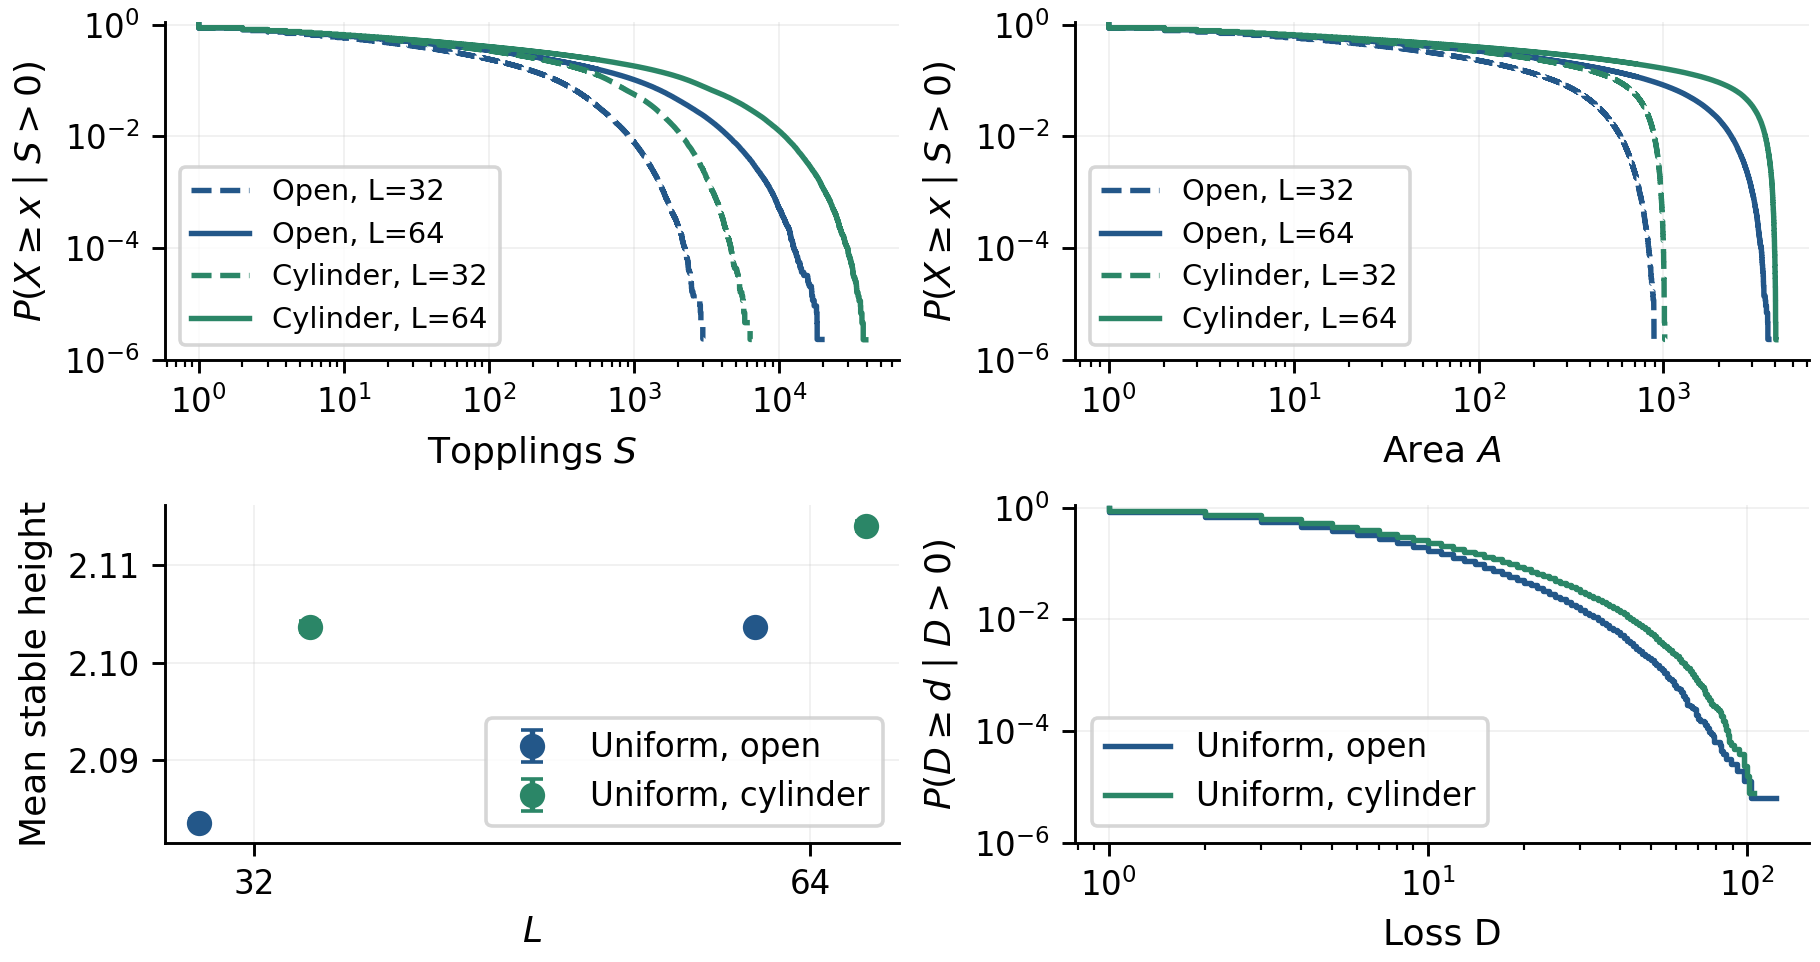
\includegraphics[width=\linewidth]{generated/cylinder.png}
\caption{Cylinder and open boundaries. Top: size and area CCDFs at $L=32,64$, conditional on $S>0$. Bottom left: mean stable height with 95\% seed intervals. Bottom right: positive-loss CCDFs at $L=64$. Each curve uses five primary seeds. Both models receive one grain per event and have theoretical mean loss one, with different loss frequencies and conditional magnitudes.}
\label{fig:cylinder}
\end{figure}

Equation~\eqref{eq:cylinder} predicts 93.5 and 357.5 topplings at $L=32,64$. The measured means are \R{cyl32S_grain} and \R{cyl64S_grain}; at $L=64$, the interval $\R{cyl64S_grainCI}$ contains the benchmark. Mean height exceeds the open control by \R{cyl64heightDifference}, interval $\R{cyl64heightDifferenceCI}$. Here the boundary change affects the height statistics as well as the response. With fewer dissipative edges, grains stay longer and generate more topplings, while conservation still fixes stationary loss at one per input. At $L=64$, mean loss is \R{cyl64D_grain}, with dissipation probability \R{cyl64p_loss} and conditional mean loss \R{cyl64D_positive}. Figure~\ref{fig:cylinder} shows how the boundary change affects size, area and loss.

\subsection{Batches as an exact grouping experiment}\label{sec:batch}
\begin{figure}[!htbp]
\centering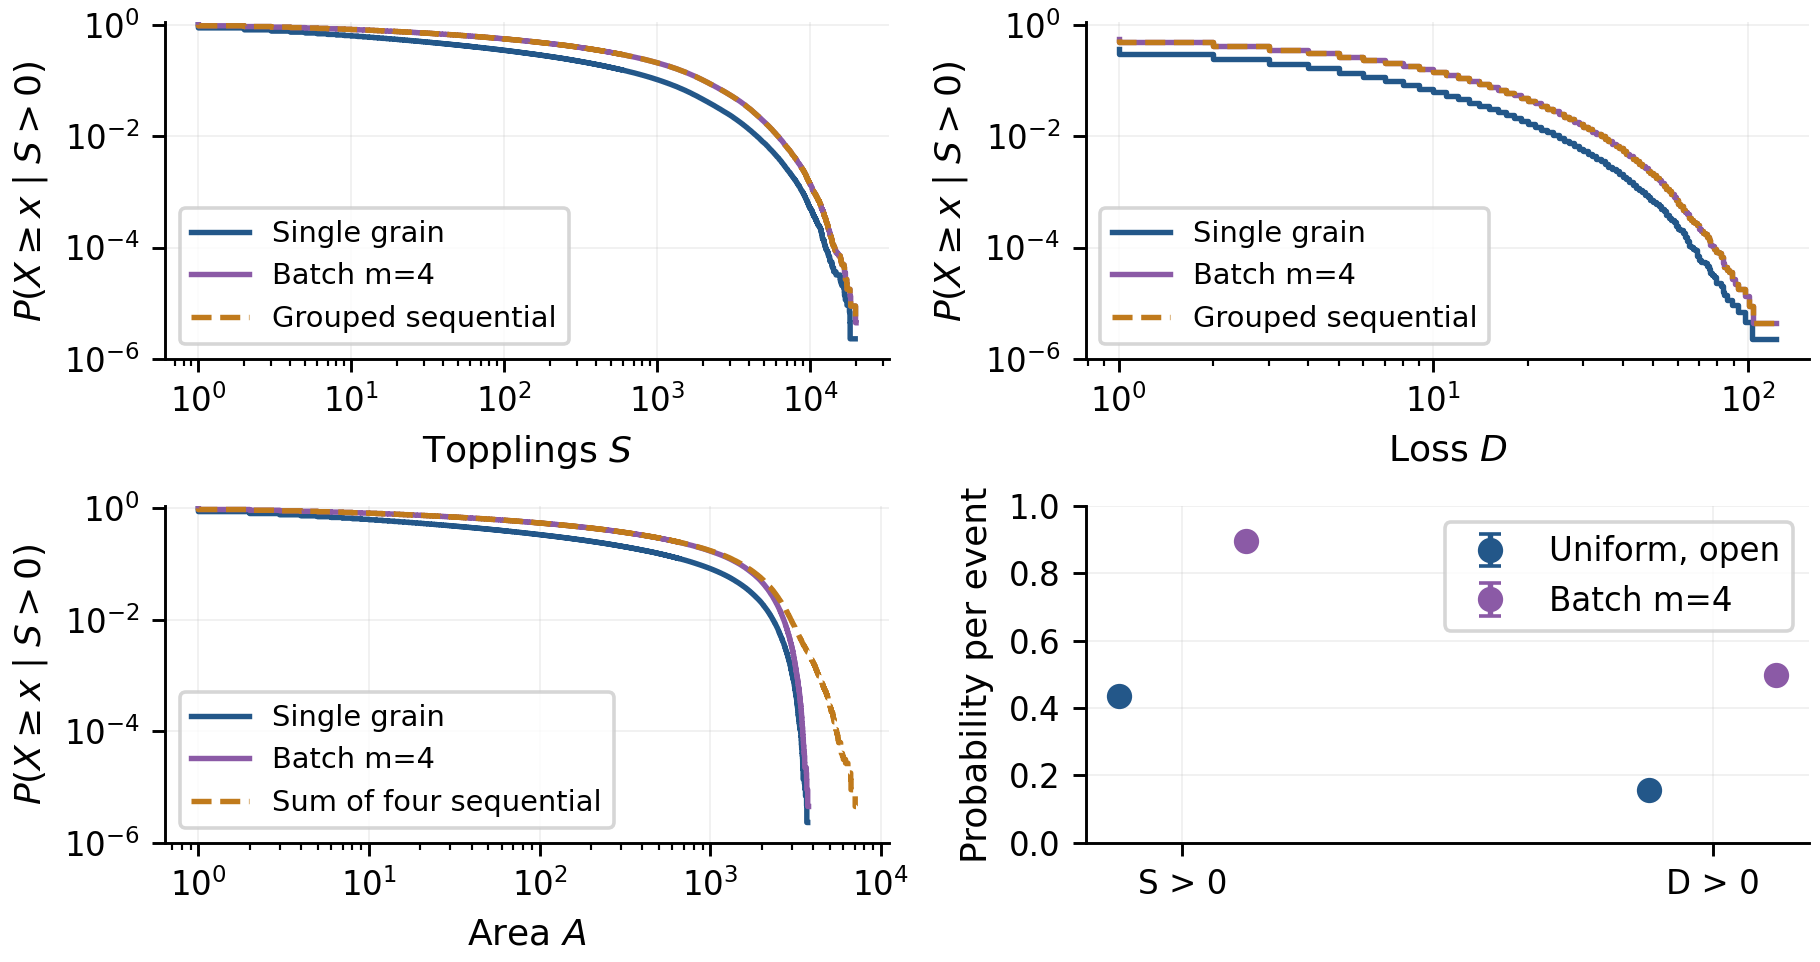
\includegraphics[width=\linewidth]{generated/batch.png}
\caption{Event grouping at $L=64$ for five matched runs: one million baseline single-grain events and 250,000 four-grain batches. Grouped sequential size and loss coincide with the batch values. For area, the third curve sums four sequential areas, counting shared sites repeatedly; the batch counts their union. Curves condition on nonzero grouped or ungrouped avalanches as appropriate. Bottom right: triggering and dissipation probabilities with seed intervals. Per-grain mean topplings and loss agree exactly in the paired runs.}
\label{fig:batch}
\end{figure}

Each batch draws four independent uniform sites with replacement and adds their grains before relaxation. We compare this with sequential single-grain additions from the same stable $h$, using the same ordered sites $s_1,\ldots,s_m$. A toppling in the sequential schedule remains legal if later, nonnegative inputs are already present. Concatenating those schedules therefore stabilizes the batched input legally. Uniqueness of the odometer gives
\begin{equation}
 h_{\rm batch}=h_{\rm sequential},\quad
 u_{\rm batch}=\sum_{r=1}^m u_r,\quad
 S_{\rm batch}=\sum_rS_r,\quad D_{\rm batch}=\sum_rD_r.\label{eq:batch}
\end{equation}
Area counts the union of toppled sites. The sum $\sum_r A_r$ counts shared sites more than once, whereas the toppling and loss identities hold even for correlated consecutive avalanches.

If $P$ is the one-grain transition, independent sources give batch transition $P^m$. Every stationary measure of $P$ is stationary for $P^m$. Depending on the sampling period, $P^m$ can still have more than one recurrent class or fail to converge from a particular start. We use a matched baseline grid after equilibration so that the comparison isolates grouping. Each batch is fully relaxed before the next one arrives.

Across both sizes, all \R{matchedBatches} batches match the grouped controls exactly in $S$, $D$ and final mass. Grid configurations and height frequencies also agree whenever sampled. Independent small-grid tests verify the full odometer and area-union identities. At $L=64$, \R{overlap64}\% of batches have overlapping toppled sets, and summing sequential areas exceeds the mean union by \R{overcount64} sites per batch. These overlaps account for the difference between the two area curves.

Grouping raises toppling probability from \R{base64p_trigger} to \R{batch64p_trigger} and loss probability from \R{base64p_loss} to \R{batch64p_loss}. Mean loss is about four per batch, with exactly the baseline value per grain. Combining successive, potentially overlapping single-grain responses changes event distributions.


